\section{Implementação numérico-computacional e resultados}

Neste capítulo, será feita uma validação numérico-computacional dos resultados analíticos obtidos nas seções anteriores empregando as técnicas do Funcional de Reciprocidade (FR) e da Transformada Integral Clássica (CITT) na estimativa da distribuição de condutância térmica de contato (CTC) ao longo de uma interface irregular segundo o arranjo proposto na figura \ref{fig2}. Este arranjo foi proposto como uma generalização da configuração estudada por \cite{tese_padilha}, na qual a interface de contato era uma superfície plana paralela às bases do corpo de prova.

Para tanto, diversos formatos de interface de contato foram propostos, bem como diferentes perfis de temperaturas medidas na superfície externa $\Gamma_0$ do corpo de prova. Para cada combinação composta por um formato de interface de contato e um perfil de temperaturas medidas na superfície externa, foi estimada, a partir das equações \eqref{calculo_FR_F1_antes}, \eqref{calculo_FR_G1_antes} e \eqref{expressao_final_ctc}, a distribuição da CTC na interface de contato referente a essa combinação, comparando-a com a distribuição de CTC teórica esperada para o caso. As medidas de temperatura na superfície externa correspondentes a uma determinada distribuição de CTC foram simuladas através da resolução do problema direto de condução de calor definido na seção \ref{sec_formulacao_direta} para a referida distribuição, e por isso são denominadas \textit{medidas sintéticas de temperatura}, ou simplesmente \textit{temperaturas sintéticas}.

Ainda seguindo a metodologia de trabalho conduzida por \cite{tese_padilha}, foram feitas simulações envolvendo erros experimentais nas medidas sintéticas de temperatura, e seus efeitos sobre a estimativa da distribuição da CTC.

\subsection{Configuração física e geométrica dos problemas-teste}\label{config_fis_geom}

Em todas as simulações, considerou-se que o corpo de prova representado na figura \ref{fig2} era composto de dois compósitos de materiais diferentes. Para o material superior $\Omega_1$ adotou-se o valor de condutividade térmica do aço AISI 1050, de 54 W/(m \celsius); para o material inferior $\Omega_2$, foi usado o valor de condutividade térmica do Incomel, de 14 W/(m \celsius). As dimensões do corpo de prova, ou seja, o comprimento e a altura da sua seção reta, foram respectivamente de 0,04 m e de 0,02 m. A superfície superior $\Gamma_0$ do corpo de prova foi submetida a um fluxo de calor por unidade de área de 100.000 W/$\text{m}^2$. Esses valores foram os mesmos adotados por \cite{tese_padilha} na condução do seu trabalho.

A Tabela \ref{tabela_params} sumariza os parâmetros físicos e geométricos usados no trabalho:
\begin{table}[h!b]
\begin{center}
	\begin{tabular}{@{}cc@{}}
		\toprule
		\textbf{Parâmetro} & \textbf{Valor}    \\ \midrule
		$a$       & 0,04 m   \\ \\
		$b$       & 0,02 m     \\ \\
		$k_1$     & 54 W/(m \celsius)  \\ \\ 
		$k_2$     & 14 W/(m \celsius) \\ \\
		$q$       & -100.000 W/$\text{m}^2$ \\ \bottomrule
	\end{tabular}		
\end{center}
\caption{Parâmetros considerados nos problemas-teste}
\label{tabela_params}
\end{table}

Foram testadas três possibilidades de geometrias de interfaces de contato. Para cada uma delas foi associada uma equação da forma $y = w(x)$, descrevendo algebricamente a curva que representa cada interface. A Tabela \ref{tabela_interfaces} apresenta a definição das expressões de cada interface de contato.
\begin{table}[h!b]
	\begin{center}
		\begin{tabular}{@{}cc@{}}
			\toprule
			\textbf{Geometria} & $w(x)$    \\ \midrule
			1       & $\displaystyle\frac{b}{2}$   \\ \\
%			2       & $\displaystyle\frac{b}{2}\left(1 + \frac{1}{5} \cos\frac{2\pi x}{a} + \frac{b}{10}\sin\frac{4\pi x}{a}\right)$     \\ \\
%			3     & $\displaystyle\frac{b}{2}\left(1 + \frac{1}{5} \sin\frac{2\pi x}{a} + \frac{b}{10}\cos\frac{4\pi x}{a}\right)$     \\ \\
			2     & $\displaystyle\frac{b}{2}\left(1 + \frac{1}{5} \cos\frac{2\pi x}{a} + \frac{1}{10}\cos\frac{4\pi x}{a}\right)$     \\ \\
%			5     & $\displaystyle \frac{b}{2}\left(\frac{3}{2} - \frac{x}{a}\right)$ \\ \\
			3       & $\displaystyle \frac{b}{2}\left(1 + \frac{1}{10} \cos\frac{5 \pi  x}{a}\right)$ \\ \bottomrule
		\end{tabular}		
	\end{center}
	\caption{Geometrias de interface de contato}
	\label{tabela_interfaces}
\end{table}
\newpage

De forma a melhor ilustrar e visualizar as diferentes geometrias de interface de contato definidas acima, as suas representações gráficas são apresentadas na Figura \ref{figura_interfaces}.
\\

\begin{figure}[h!b]
	\begin{minipage}[t][5cm][c]{\textwidth}
		\centering
		\begin{tikzpicture}
			\begin{axis}[
			anchor=east,  
			ticks=none,
			width=8cm,
			height=4cm,
			%ylabel=Iterações Lineares,
			xmin = 0,
			xmax = 0.04,
			ymin = 0,
			ymax = 0.02]
			\pgfplotstableread{../data/interface_01.dat} 
			\teff
			\addplot[color=blue,mark=none,smooth] table from \teff;
			\end{axis}
		\end{tikzpicture}
		\caption*{(a) Geometria 1}
	\end{minipage}
%	\begin{minipage}[t][5cm][t]{0,5\textwidth}
%		\begin{tikzpicture}
%		\begin{axis}[
%		anchor=east,  
%		ticks=none,
%		width=8cm,
%		height=4cm,
%		%ylabel=Iterações Lineares,
%		xmin = 0,
%		xmax = 0.04,
%		ymin = 0,
%		ymax = 0.02]
%		\pgfplotstableread{../data/interface_05.dat} 
%		\teff
%		\addplot[color=blue,mark=none,smooth] table from \teff;
%		\end{axis}
%		\end{tikzpicture}
%		\caption*{(b) Geometria 2}
%	\end{minipage}
%	\begin{minipage}[t][5cm][t]{0,5\textwidth}
%		\begin{tikzpicture}
%		\begin{axis}[
%		anchor=east,  
%		ticks=none,
%		width=8cm,
%		height=4cm,
%		%ylabel=Iterações Lineares,
%		xmin = 0,
%		xmax = 0.04,
%		ymin = 0,
%		ymax = 0.02]
%		\pgfplotstableread{../data/interface_06.dat} 
%		\teff
%		\addplot[color=blue,mark=none,smooth] table from \teff;
%		\end{axis}
%		\end{tikzpicture}
%		\caption*{(c) Geometria 3}
%	\end{minipage}
	\begin{minipage}[t][5cm][c]{\textwidth}
		\centering
		\begin{tikzpicture}
		\begin{axis}[
		anchor=east,  
		ticks=none,
		width=8cm,
		height=4cm,
		%ylabel=Iterações Lineares,
		xmin = 0,
		xmax = 0.04,
		ymin = 0,
		ymax = 0.02]
		\pgfplotstableread{../data/interface_02.dat} 
		\teff
		\addplot[color=blue,mark=none,smooth] table from \teff;
		\end{axis}
		\end{tikzpicture}
		\caption*{(d) Geometria 2}
	\end{minipage}
%	\begin{minipage}[t][5cm][t]{0,5\textwidth}
%		\begin{tikzpicture}
%		\begin{axis}[
%		anchor=east,  
%		ticks=none,
%		width=8cm,
%		height=4cm,
%		%ylabel=Iterações Lineares,
%		xmin = 0,
%		xmax = 0.04,
%		ymin = 0,
%		ymax = 0.02]
%		\pgfplotstableread{../data/interface_08.dat} 
%		\teff
%		\addplot[color=blue,mark=none,smooth] table from \teff;
%		\end{axis}
%		\end{tikzpicture}
%		\caption*{(e) Geometria 5}
%	\end{minipage}
	\begin{minipage}[t][5cm][c]{\textwidth}
		\centering
		\begin{tikzpicture}
		\begin{axis}[
		anchor=east,  
		ticks=none,
		width=8cm,
		height=4cm,
		%ylabel=Iterações Lineares,
		xmin = 0,
		xmax = 0.04,
		ymin = 0,
		ymax = 0.02]
		\pgfplotstableread{../data/interface_03.dat} 
		\teff
		\addplot[color=blue,mark=none,smooth] table from \teff;
		\end{axis}
		\end{tikzpicture}
		\caption*{(f) Geometria 3}
	\end{minipage}	
	\caption{Diferentes geometrias para a interface $\Gamma$}
	\label{figura_interfaces}
\end{figure}

\subsection{Perfis teóricos de condutância térmica de contato}\label{config_ctc}

Foram adotados três diferentes perfis de distribuição de CTC, extraídos do trabalho de \cite{tese_padilha} e trabalhos anteriores. Estes perfis estão listados na Tabela \ref{tabela_ctc}, onde $h_{max}$ corresponde ao valor máximo que a CTC pode assumir, fixado em 1000 W/($\text{m}^2$ \celsius), e $a$ é o comprimento do corpo de prova.
\newpage
\begin{table}[h!b]
	\begin{center}
		\begin{tabular}{c|c}
			\hline \\
			\textbf{Perfil} & $h_c(x)$[W/($\text{m}^2$ \celsius)]  \\ \\ \hline \\
			\multirow{2}{*}{1} & $h_{max}$ para $x < a/4$ e $x > 3a/4$ \\ & 0 para $a/4 < x < 3a/4$ \\ \\ \hline \\
%			\multirow{2}{*}{2} & $h_{max}$ para $x < a/4$ e $a/2 < x < 3a/4$ \\ & 0 para $a/4 < x < a/2$ e $x > 3a/4$ \\ \\ \hline \\
			2 & $h_{max}\sin\displaystyle\frac{\pi x}{a}$ \\ \\ \hline \\
%			4 & $\abs{h_{max}\sin\displaystyle\frac{2\pi x}{a}}$ \\ \\ \hline \\
%			5 & $h_{max}$ \\ \\ \hline \\
			\multirow{3}{*}{3} & $h_{max}/2$ para $x < a/4$ e $a/2 < x < 3a/4$ \\ & $h_{max}$ para $a/4 < x < a/2$ \\ & 0 para $ x > 3a/4$
			\\ \\ \hline
		\end{tabular}		
	\end{center}
	\caption{Geometrias de interface de contato}
	\label{tabela_ctc}
\end{table}

De forma a melhor ilustrar e visualizar os diferentes perfis definidos acima, as suas representações gráficas são apresentadas na Figura \ref{figura_ctc}.
\begin{figure}[h!b]
	\begin{minipage}[t][5cm][c]{\textwidth}
		\centering		
		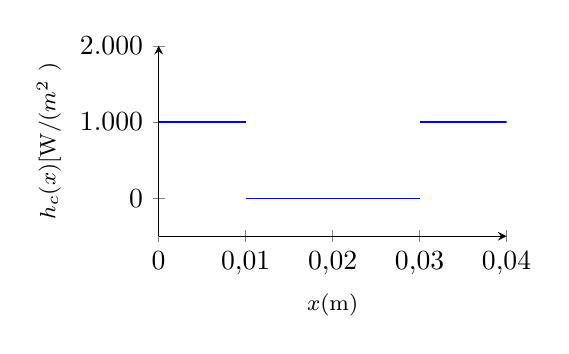
\begin{tikzpicture}
		\begin{axis}[
		/pgf/number format/1000 sep={.},/pgf/number format/use comma,
		axis lines=left,
		xmin = 0,
		xmax = 0.04,
		ymin = -500,
		ymax = 2000,
		restrict y to domain=-500:2000,
		scaled x ticks = false,
		scaled y ticks = false,
		x tick label style={/pgf/number format/fixed},
		y tick label style={/pgf/number format/fixed},
		anchor=east,  
		width=6cm,
		height=4cm,
		label style={font=\footnotesize},
		xlabel = $x$(m),
		ylabel= $h_c(x)[$W/($\text{m}^2$ \celsius)]]
		\addplot[color=blue,mark=none,smooth, domain=0:0.01] {1000};
		\addplot[color=blue,mark=none,smooth, domain=0.01:0.03] {0};
		\addplot[color=blue,mark=none,smooth, domain=0.03:0.04] {1000};
		\end{axis}
		\end{tikzpicture}
		\caption*{(a) Perfil 1}
	\end{minipage}
\end{figure}
%	\begin{minipage}[t][5cm][t]{0,5\textwidth}
%		\begin{tikzpicture}
%		\begin{axis}[
%		axis lines=left,
%		xmin = 0,
%		xmax = 0.04,
%		ymin = -500,
%		ymax = 2000,
%		restrict y to domain=-500:2000,
%		scaled x ticks = false,
%		scaled y ticks = false,
%		x tick label style={/pgf/number format/fixed},
%		y tick label style={/pgf/number format/fixed},
%		anchor=east,  
%		width=6cm,
%		height=4cm,
%		label style={font=\footnotesize},
%		xlabel = $x$(m),
%		ylabel= $h_c(x)$[W/($\text{m}^2$ \celsius)]]
%		\pgfplotstableread{../data/conductance_02.dat} 
%		\teff
%		\addplot[color=blue,mark=none,smooth] table from \teff;
%		\end{axis}
%		\end{tikzpicture}
%		\caption*{(a) Perfil 2}
%	\end{minipage}
\begin{figure}[h!b]
	\begin{minipage}[t][5cm][c]{\textwidth}
		\centering
		\begin{tikzpicture}
		\begin{axis}[
		/pgf/number format/1000 sep={.},/pgf/number format/use comma,
		axis lines=left,
		xmin = 0,
		xmax = 0.04,
		ymin = -500,
		ymax = 2000,
		restrict y to domain=-500:2000,
		scaled x ticks = false,
		scaled y ticks = false,
		x tick label style={/pgf/number format/fixed},
		y tick label style={/pgf/number format/fixed},
		anchor=east,  
		width=6cm,
		height=4cm,
		label style={font=\footnotesize},
		xlabel = $x$(m),
		ylabel= $h_c(x)$[W/($\text{m}^2$ \celsius)]]
		\pgfplotstableread{../data/conductance_02.dat} 
		\teff
		\addplot[color=blue,mark=none,smooth] table from \teff;
		\end{axis}
		\end{tikzpicture}
		\caption*{(a) Perfil 2}
	\end{minipage}
\end{figure}
\newpage
%	\begin{minipage}[t][5cm][t]{0,5\textwidth}
%		\begin{tikzpicture}
%		\begin{axis}[
%		axis lines=left,
%		xmin = 0,
%		xmax = 0.04,
%		ymin = -500,
%		ymax = 2000,
%		restrict y to domain=-500:2000,
%		scaled x ticks = false,
%		scaled y ticks = false,
%		x tick label style={/pgf/number format/fixed},
%		y tick label style={/pgf/number format/fixed},
%		anchor=east,  
%		width=6cm,
%		height=4cm,
%		label style={font=\footnotesize},
%		xlabel = $x$(m),
%		ylabel= $h_c(x)$[W/($\text{m}^2$ \celsius)]]
%		\pgfplotstableread{../data/conductance_04.dat} 
%		\teff
%		\addplot[color=blue,mark=none,smooth] table from \teff;
%		\end{axis}
%		\end{tikzpicture}
%		\caption*{(a) Perfil 4}
%	\end{minipage}
%	\begin{minipage}[t][5cm][t]{0,5\textwidth}
%		\begin{tikzpicture}
%		\begin{axis}[
%		axis lines=left,
%		xmin = 0,
%		xmax = 0.04,
%		ymin = -500,
%		ymax = 2000,
%		restrict y to domain=-500:2000,
%		scaled x ticks = false,
%		scaled y ticks = false,
%		x tick label style={/pgf/number format/fixed},
%		y tick label style={/pgf/number format/fixed},
%		anchor=east,  
%		width=6cm,
%		height=4cm,
%		label style={font=\footnotesize},
%		xlabel = $x$(m),
%		ylabel= $h_c(x)$[W/($\text{m}^2$ \celsius)]]
%		\pgfplotstableread{../data/conductance_05.dat} 
%		\teff
%		\addplot[color=blue,mark=none,smooth] table from \teff;
%		\end{axis}
%		\end{tikzpicture}
%		\caption*{(a) Perfil 5}
%	\end{minipage}
\begin{figure}[h!b]
	\begin{minipage}[t][5cm][c]{\textwidth}
		\centering
		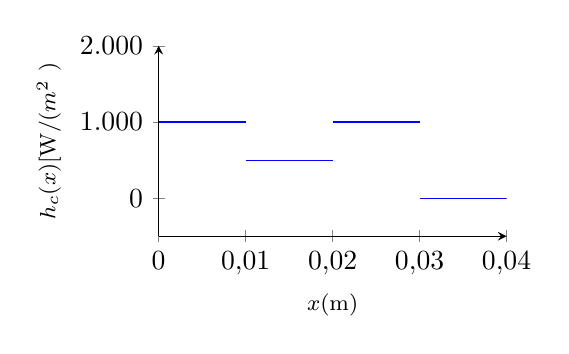
\begin{tikzpicture}
		\begin{axis}[
		/pgf/number format/1000 sep={.},/pgf/number format/use comma,
		axis lines=left,
		xmin = 0,
		xmax = 0.04,
		ymin = -500,
		ymax = 2000,
		restrict y to domain=-500:2000,
		scaled x ticks = false,
		scaled y ticks = false,
		x tick label style={/pgf/number format/fixed},
		y tick label style={/pgf/number format/fixed},
		anchor=east,  
		width=6cm,
		height=4cm,
		label style={font=\footnotesize},
		xlabel = $x$(m),
		ylabel= $h_c(x)$[W/($\text{m}^2$ \celsius)]]
		\addplot[color=blue,mark=none,smooth, domain=0:0.01] {1000};
		\addplot[color=blue,mark=none,smooth, domain=0.01:0.02] {500};
		\addplot[color=blue,mark=none,smooth, domain=0.02:0.03] {1000};
		\addplot[color=blue,mark=none,smooth, domain=0.03:0.04] {0};
		\end{axis}
		\end{tikzpicture}
		\caption*{(a) Perfil 3}
	\end{minipage}	
	\caption{Diferentes perfis de $h_c(x)$ na interface $\Gamma$}
	\label{figura_ctc}
\end{figure}


\subsection{Determinação das temperaturas sintéticas}

As medidas de temperatura na superfície superior $\Gamma_0$ do corpo de prova, representadas por $Y$ nas expressões \eqref{calculo_FR_F1_antes} e \eqref{calculo_FR_G1_antes}, foram obtidas resolvendo o problema direto definido na seção \ref{sec_formulacao_direta}, com os parâmetros, perfis de CTC e geometrias de interface indicados nas seções \ref{config_fis_geom} e \ref{config_ctc}. A fim de evitar a ocorrência do ``crime inverso", isto é, uma redução artificial do mal condicionamento do problema inverso quando o método empregado para resolvê-lo é o mesmo aplicado ao problema direto que fornece as medidas sintéticas\citep{livro_kaipio}, foram executadas simulações das diferentes configurações do problema direto no COMSOL \textit{Multiphysics}\textsuperscript{\textregistered}. O COMSOL é um \textit{software} comercial de elementos finitos, que possui um módulo específico para simulações de transferência de calor.

As várias configurações possíveis do problema direto definido na seção \ref{sec_formulacao_direta} foram modeladas e simuladas neste programa, seguindo os dados apresentados nas tabelas \ref{tabela_params}, \ref{tabela_interfaces} e \ref{tabela_ctc}, usando uma malha triangular extrafina. Para cada configuração, os valores de temperatura ao longo da interface superior $\Gamma_0$ foram exportados em arquivos-texto e usados como entrada para o programa implementado para a estimativa da CTC, e que será comentado na seção \ref{sobre_o_programa}. Convencionou-se extrair um total de 120 pontos equidistantes de medição de temperatura sobre a superfície $\Gamma_0$ para cada configuração.

Para fins de verificação, as mesmas combinações foram resolvidas numericamente através do método da Transformada Integral Clássica, e os resultados obtidos para a distribuição de temperaturas sobre a superfície $\Gamma_0$ apresentaram boa aderência com os obtidos a partir do COMSOL. A título de exemplo, as figuras \ref{fig_comparativo_1} e \ref{fig_comparativo_2} apresentam, respectivamente, um comparativo entre as temperaturas levantadas na superfície superior do corpo de prova, para a configuração específica referente à interface 3 e condutância de contato 1, e a distribuição do desvio relativo percentual entre essas medidas, calculada por:
\begin{align}
\epsilon_i = 100\abs{\frac{T\textsuperscript{COMSOL}_i - T\textsuperscript{CITT}_i}{T\textsuperscript{COMSOL}_i}}, i \in \Gamma_0
\end{align}

\begin{figure}[h!b]
	\begin{minipage}[t][8cm][c]{\textwidth}
		\centering
		\begin{tikzpicture}
		\begin{axis}[
		/pgf/number format/1000 sep={.},/pgf/number format/use comma,
		axis lines=left,
		%		xmin = 0,
		%		xmax = 0.04,
		%		ymin = 310,
		%		ymax = 340,
		%		restrict y to domain=-500:2000,
		scaled x ticks = false,
		scaled y ticks = false,
		x tick label style={/pgf/number format/fixed},
		y tick label style={/pgf/number format/fixed},
		anchor=east,  
		width=7cm,
		height=5cm,
		label style={font=\footnotesize},
		xlabel = $x$(m),
		ylabel= $T_1\big|_{\Gamma_0}$ (\celsius)]
		\pgfplotstableread{../data/fortran/temperaturas_sinteticas_interface_03_conductance_01.dat} 
		\teff
		\addplot[color=blue,mark=o,mark options={mark size=1.0pt}] table from \teff;
		\pgfplotstableread{../data/comsol/temperaturas_sinteticas_interface_03_conductance_01.dat} 
		\teff
		\addplot[only marks,color=red,mark=square,mark options={mark size=1.0pt}] table from \teff;
		\end{axis}
		\end{tikzpicture}
		\caption{Temperatura na superfície superior $\Gamma_0$ para a configuração referente à interface 3 e condutância de contato 1: $\textcolor{blue}{\ocircle} \rightarrow$ CITT; $\textcolor{red}{\square} \rightarrow$ Elementos finitos (COMSOL)}
		\label{fig_comparativo_1}
	\end{minipage}
	\begin{minipage}[t][8cm][c]{\textwidth}
		\centering
		\begin{tikzpicture}
		\begin{axis}[
		/pgf/number format/1000 sep={.},/pgf/number format/use comma,
		axis lines=left,
		%		xmin = 0,
		%		xmax = 0.04,
				ymin = 0.085,
				ymax = 0.105,
		%		restrict y to domain=-500:2000,
		scaled x ticks = false,
		scaled y ticks = false,
		x tick label style={/pgf/number format/fixed},
		y tick label style={/pgf/number format/fixed, /pgf/number format/precision=5},
		anchor=east,  
		width=7cm,
		height=5cm,
		label style={font=\footnotesize},
		xlabel = $x$(m),
		ylabel= $\epsilon$ (\%)]
		\pgfplotstableread{../data/desvio_relativo_interface_03_conductance_01.dat} 
		\teff
		\addplot[mark=o,mark options={mark size=1.0pt}] table from \teff;
		\end{axis}
		\end{tikzpicture}
		\caption{Desvio percentual entre as temperaturas obtidas via CITT e método dos elementos finitos (COMSOL), na superfície superior $\Gamma_0$ para a configuração referente à interface 3 e condutância de contato 1}
		\label{fig_comparativo_2}
	\end{minipage}
\end{figure}

As temperaturas sintéticas obtidas a partir do COMSOL correspondem a medidas consideradas exatas, sem ruídos ou erros experimentais. De forma a simular medidas com erros experimentais, foi implementado o mesmo procedimento adotado por \cite{tese_padilha}: foram adicionados erros randômicos com distribuição normal às temperaturas calculadas sobre a superfície superior do corpo de prova. Sendo então $\mathbf{Y}$ as medidas de temperatura simuladas sem erros, as medidas simuladas com erros, denotadas por $\tilde{\mathbf{Y}}$, foram calculadas através da expressão:
\begin{align}
\tilde{\mathbf{Y}} = \mathbf{Y} + \mathbf{\varepsilon} \sigma \label{modelagem_erro}
\end{align}
onde $\sigma$ é o desvio padrão das medidas de temperatura, e $\varepsilon$ é uma sequência aleatória gerada a partir da transformação Box-Muller\citep{artigo_box_muller}:
\begin{align}
\varepsilon = \cos(2\pi v)\sqrt{-2 \ln u}
\end{align}
onde $u$ e $v$ correspondem a variáveis aleatórias contínuas com distribuição uniforme entre 0 e 1.

Três níveis de desvio-padrão foram testados: $\sigma = \text{0,0}\celsius$ (correspondente aos casos onde as temperaturas sintéticas não contém erros), $\sigma = \text{0,1}\celsius$ e $\sigma = \text{0,5}\celsius$. Desse modo, havendo três possibilidades de geometrias de interface de contato e três possibilidades de condutância térmica de contato teórica, foram realizadas nove simulações distintas de problemas-teste diretos, para obtenção das respectivas distribuições de temperaturas sintéticas exatas. A cada um desses resultados foram aplicados os erros correpondentes às três possibilidades de desvio-padrão, num total de 27 conjuntos de dados de entrada; estes dados por sua vez alimentaram cada um dos 27 problemas inversos equivalentes resolvidos neste trabalho. Nas figuras \ref{figura_temperaturas_sinteticas_interface_01}, \ref{figura_temperaturas_sinteticas_interface_02} e \ref{figura_temperaturas_sinteticas_interface_03}, é possível visualizar as distribuições de temperaturas sintéticas na superfície superior do corpo de prova para cada uma das configurações. A maior ou menor dispersão dos dados com erros aleatórios em torno das medidas exatas é devida apenas às diferentes escalas adotadas no eixo $y$ de cada gráfico.
\newpage

%%%%%%%%%%%%%%%%%%%%%%%%%
% Temperaturas em y = b
%%%%%%%%%%%%%%%%%%%%%%%%%

% indice da interface
% indice da condutancia
\newcommand{\graficostemperatura}[3]{%
	\begin{minipage}[t][6cm][c]{4.5cm}
		\centering		
		\begin{tikzpicture}[scale=0.75]
		\begin{axis}[
		/pgf/number format/1000 sep={.},/pgf/number format/use comma,
		axis lines=left,
		%		xmin = 0,
		%		xmax = 0.04,
		%		ymin = 310,
		%		ymax = 340,
		%		restrict y to domain=-500:2000,
		scaled x ticks = false,
		scaled y ticks = false,
		x tick label style={/pgf/number format/fixed},
		y tick label style={/pgf/number format/fixed},
		anchor=east,  
		width=7cm,
		height=5cm,
		label style={font=\footnotesize},
		xlabel = $x$(m),
		ylabel= $T_1\big|_{\Gamma_0}$ (\celsius),
		ylabel style={rotate=-90, at={(-0.1, 1)}, anchor = south west}]		
		\pgfplotstableread{../data/temperaturas_sinteticas_interface_0#1_conductance_0#2_stdev_05.dat} 
		\teff
		\addplot[only marks,color=gray,mark=triangle,mark options={mark size=2.0pt}] table from \teff;
		\pgfplotstableread{../data/temperaturas_sinteticas_interface_0#1_conductance_0#2_stdev_01.dat} 
		\teff
		\addplot[only marks,color=red,mark=square,mark options={mark size=2.0pt}] table from \teff;
		\pgfplotstableread{../data/temperaturas_sinteticas_interface_0#1_conductance_0#2_stdev_00.dat} 
		\teff
		\addplot[color=blue,mark=o,mark options={mark size=2.0pt}] table from \teff;		
		\end{axis}
		\end{tikzpicture}
		\caption*{(#3) Perfil #2}
	\end{minipage}
}%

%%%%%%%%%%%%%%%%%%%%%%%%%
%%%%TODO apenas para acelerar a compilação
%%%%%%%%%%%%%%%%%%%%%%%%

%\begin{figure}[h!b]
%	\graficostemperatura{1}{1}{a}
%	\graficostemperatura{1}{2}{b}
%	\graficostemperatura{1}{3}{c}
%	\caption{Temperaturas sintéticas ($Y$) ao longo da superfície superior $\Gamma_0$, para os perfis de CTC de 1 a 3, referentes à interface de contato 1: $\textcolor{blue}{\ocircle} \rightarrow \sigma = 0.0$; $\textcolor{red}{\square} \rightarrow \sigma = 0.1$, $\textcolor{gray}{\triangle} \rightarrow \sigma = 0.5$}
%	\label{figura_temperaturas_sinteticas_interface_01}
%\end{figure}
%\begin{figure}[h!b]
%	\graficostemperatura{2}{1}{a}
%	\graficostemperatura{2}{2}{b}
%	\graficostemperatura{2}{3}{c}
%	\caption{Temperaturas sintéticas ($Y$) ao longo da superfície superior $\Gamma_0$, para os perfis de CTC de 1 a 3, referentes à interface de contato 2: $\textcolor{blue}{\ocircle} \rightarrow \sigma = 0.0$; $\textcolor{red}{\square} \rightarrow \sigma = 0.1$, $\textcolor{gray}{\triangle} \rightarrow \sigma = 0.5$}
%	\label{figura_temperaturas_sinteticas_interface_02}
%\end{figure}
%\begin{figure}[h!b]
%	\graficostemperatura{3}{1}{a}
%	\graficostemperatura{3}{2}{b}
%	\graficostemperatura{3}{3}{c}
%	\caption{Temperaturas sintéticas ($Y$) ao longo da superfície superior $\Gamma_0$, para os perfis de CTC de 1 a 3, referentes à interface de contato 3: $\textcolor{blue}{\ocircle} \rightarrow \sigma = 0.0$; $\textcolor{red}{\square} \rightarrow \sigma = 0.1$, $\textcolor{gray}{\triangle} \rightarrow \sigma = 0.5$}
%	\label{figura_temperaturas_sinteticas_interface_03}
%\end{figure}

\subsection{Código computacional}\label{sobre_o_programa}

Neste trabalho, o código computacional foi desenvolvido usando a linguagem de programação Fortran 2003. O compilador usado foi o \textit{gfortran}, que faz parte do projeto de \textit{software} livre GCC. O ambiente de desenvolvimento, onde o código era editado, compilado e depurado, foi o Eclipse, que também é um \textit{software} não-comercial. Todo o trabalho foi desenvolvido num computador executando o sistema operacional Linux para plataforma de 64 bits; no caso, a distribuição do sistema operacional usada foi Ubuntu versão 16.04.

As rotinas numéricas empregadas foram obtidas do projeto Netlib\footnote{Mais informações sobre o repositório Netlib podem ser encontradas no endereço de Internet \href{https://www.netlib.org/}{https://www.netlib.org/}.}, que é um repositório \textit{online} mantido por algumas instituições e universidades, contendo \textit{software} de computação científica e documentação disponíveis gratuitamente. A maioria das rotinas encontradas no repositório Netlib está escrita em FORTRAN 77\footnote{O uso de caixa alta para designar a versão 77 da linguagem Fortran tem raízes históricas, sendo encontrado em muitas publicações, e por isso esta convenção foi mantida aqui.}, especialmente as usadas no programa desenvolvido para este trabalho, o que não trouxe dificuldades, pois o compilador \textit{gfortran} é capaz de efetuar a compilação híbrida de arquivos-fonte escritos tanto em FORTRAN 77 quanto em Fortran 2003, inclusive padronizando para que todas as variáveis de ponto flutuante de precisão simples sejam tratadas como sendo de precisão dupla, o que de fato foi feito no programa.
A livre disponibilidade do código-fonte das rotinas facilitou significativamente a depuração do programa e a consequente identificação e correção de erros, sendo um fator determinante no desenvolvimento do mesmo. 

Foram empregadas rotinas numéricas do repositório Netlib para realizar as seguintes tarefas:
\begin{itemize}
	\item Cálculo das integrais presentes nas equações \eqref{calculo_FR_F1_antes} e \eqref{calculo_FR_G1_antes}. Estas integrais são da forma
	\begin{align}
	& \int_0^a Y(x)dx \\ \nonumber \\
	& \int_0^a Y(x)\cos\mu_m x dx
	\end{align}
	Estas integrais devem ser resolvidas numericamente, uma vez que o termo $Y(x)$, referente às temperaturas sintéticas sobre a superfície superior do corpo de prova, corresponde na verdade a um conjunto de dados discretos cuja formulação analítica é desconhecida (num problema real). Foram utilizadas duas rotinas que trabalhavam em conjunto: CURFIT, que aproxima um conjunto de pontos $(x_i, y_i)$ em uma B-\textit{spline}, e SPLINT, que integra a B-\textit{spline} obtida da rotina anterior sobre um intervalo.
	
	\item Cálculo das transformadas integrais que fornecem os coeficientes dos sistemas lineares \eqref{sistema_para_coeficientes_3} e \eqref{sistema_para_coeficientes_21}. O repositório Netlib oferece a rotina DQAWO, que faz parte do subprojeto QUADPACK, e que resolve integrais da forma
	\begin{align}
	& \int_{x_0}^{x_1} f(x)\cos\omega x dx \label{dqawo} \\ \nonumber \\
	& \int_{x_0}^{x_1} f(x)\sin\omega x dx 
	\end{align}
	A rotina foi parametrizada para resolver integrais conforme a expressão \eqref{dqawo}, fazendo $\omega = \mu_m$.
	
	\item Solução numérica dos sistemas de equações lineares \eqref{sistema_para_coeficientes_3} e \eqref{sistema_para_coeficientes_21}. O repositório Netlib possui o subprojeto LAPACK (\textit{Linear Algebra PACKage}), contendo diversos \textit{solvers} de sistemas lineares para várias possibilidades de matrizes de coeficientes: matrizes-banda, simétricas, positivas definidas, etc, além de outros utilitários de Álgebra Linear. A rotina DGESVX, utilizada no trabalho, recebe como entrada a matriz de coeficientes e uma matriz cujas colunas são diferentes vetores de termos independentes do sistema; a rotina aplica um pré-condicionador ao sistema, realiza uma decomposição LU da matriz de coeficientes e usa este resultado para obter os vetores-solução referentes a cada vetor de termos independentes. Esta rotina atendeu à necessidade de se resolver de forma eficiente um dado sistema de equações, variando apenas o segundo membro correspondente aos termos independentes, o que foi comentado na seção \ref{orto_beta_gama}.
	
	\item Cálculo das integrais necessárias para a ortogonalização de Gram-Schmidt. Estas integrais, definidas de forma geral pela equação \eqref{integral_da_definicao_produto_interno_4}, foram calculadas através da rotina de integração de propósito geral DAQG, que realiza uma integração adaptativa através das fórmulas de quadratura de Gauss-Konrod.
\end{itemize}

\subsection{Resultados e análises}

Serão apresentados agora os resultados numéricos obtidos a partir da aplicação das equações \eqref{calculo_FR_F1_antes}, \eqref{calculo_FR_G1_antes} e \eqref{expressao_final_ctc} ao problema inverso de condução de calor descrito na seção \ref{sec_prob_inv}. Estas equações fornecem, respectivamente, as estimativas de salto de temperatura, fluxo de calor e condutância térmica de contato na interface entre os materiais que compõem o arranjo físico ilustrado na figura \ref{fig2}.

Para cada combinação possível de geometria de interface (tabela \ref{tabela_interfaces}), perfil de condutância térmica de contato (tabela \ref{tabela_ctc}) e desvio-padrão de erros de medição ($\sigma = \text{0,0}\celsius$, $\sigma = \text{0,1}\celsius$ e $\sigma = \text{0,5}\celsius$), foram calculadas estimativas de salto de temperatura e fluxo de calor na interface de contato, e os resultados foram comparados com os respectivos valores teóricos esperados para cada combinação. A estimativa do perfil de condutância térmica de contato, calculada através da razão entre o salto de temperartura e fluxo de calor estimados na interface, também foi comparada com o perfil teórico correspondente, e que foi usado para determinação prévia das temperaturas sintéticas através de simulações de cada configuração do problema no módulo de transferência de calor no simulador COMSOL \textit{Multiphysics}\textsuperscript{\textregistered}.

Todas as combinações analisadas são, de certo modo, condições ideais, no sentido de que a solução exata esperada para cada problema-teste já era previamente conhecida. Num problema real, entretanto, a distribuição da condutância térmica de contato ao longo da interface $\Gamma$ é desconhecida -- com efeito, trata-se da função que se deseja estimar -- tampouco se conhece a distribuição do salto de temperatura e do fluxo de calor naquela interface. Estes últimos parâmetros foram estimados a partir de dois somatórios envolvendo os funcionais de reciprocidade (equações \eqref{resultado_1} e \eqref{resultado_2}), ou seja:
\begin{align}
[T_1 - T_2]_\Gamma = \sum_{j=1}^{N_1} k_1 \Re(F_{1,j}) \beta_j \label{resultado_1_again} \\ \nonumber \\
- k_1 \frac{\partial T_1}{\partial\mathbf{n_1}}\bigg|_\Gamma = \sum_{j=1}^{N_2} k_1 \Re(G_{1,j}) \gamma_j \label{resultado_2_again}
\end{align}

Em teoria, quanto maiores fossem os limites dos somatórios $N_1$ e $N_2$, melhores seriam as estimativas fornecidas de salto de temperatura e fluxo de calor. No desenvolvimento deste trabalho, porém, observou-se que esse padrão era seguido até algum número máximo de termos nos somatórios \eqref{resultado_1_again} e \eqref{resultado_2_again}, a partir do qual as estimativas afastavam-se cada vez mais dos valores exatos correspondentes. Ou seja, ao contrário do que normalmente se observa numa série numérica, um incremento na quantidade de parcelas a serem somadas naquelas expressões não implicava obrigatoriamente numa tendência consistente de convergência do somatório para um valor finito.

Foi necessário, portanto, estabelecer um critério para determinação do número máximo de parcelas nos somatórios que representavam as estimativas. Para levantamento desse número ótimo de termos, foi adotada neste trabalho a proposta apresentada por \cite{tese_padilha}, que empregou, como métrica de avaliação da qualidade da estimativa, uma norma baseada nas diferenças entre duas estimativas sucessivas ao longo da superfície $\Gamma$:

%Muito embora os resultados numéricos obtidos para as estimativas de CTC em cada um dos casos discutidos nas seções anteriores só sejam apresentados posteriormente neste trabalho, cabe aqui comentar aspectos referentes a uma característica notável do problema inverso de condução de calor estudado, qual seja, o comportamento instável da estimativa do salto de temperatura e do fluxo de calor na interface $\Gamma$ (vide Figura \ref{fig2}) em relação à quantidade de termos $N_1$ e $N_2$ usados nas suas respectivas expansões em somatórios de combinações lineares de funcionais de reciprocidade, deduzidas na seção \ref{secao_sobre_fr}:
%\begin{align}
%& [T_1 - T_2]_\Gamma = \sum_{j=1}^{N_1} k_1 \Re(F_{1,j}) \beta_j \label{resultado_1_rep} \\ \nonumber \\
%& - k_1 \frac{\partial T_1}{\partial\mathbf{n_1}}\bigg|_\Gamma = \sum_{j=1}^{N_2} k_1 \Re(G_{1,j}) \gamma_j \label{resultado_2_rep}
%\end{align}
%
%No trabalho de \cite{tese_padilha}, foram obtidos, a partir da solução do problema direto para o caso da interface de contato plana e horizontal, a distribuição teórica do salto de temperatura e do fluxo de calor ao longo da interface $\Gamma$ para cada problema-teste. As expressões 
%\eqref{resultado_1_rep} e \eqref{resultado_2_rep} foram usadas naquele trabalho para estimativa do salto de temperatura e do fluxo de calor na interface, da mesma maneira como foi realizado no trabalho corrente, com a diferença de que a determinação dos funcionais de reciprocidade $\Re(F_{1,j})$ e $\Re(G_{1,j})$ era puramente analítica, sem a etapa de resolução de sistemas lineares como os obtidos nas seções \ref{secao_reciprocidade_F} e \ref{secao_reciprocidade_G}. Foram empregadas as seguintes expressões para o erro da raiz média quadrática (RMS) entre os resultados exatos e os estimados \footnote{A notação adotada por \cite{tese_padilha} na representação destas expressões era bem mais simples; porém as expressões aqui apresentadas são mais gerais e se reduzem facilmente à formulação usada naquele trabalho.}:
%\begin{align}
%& \delta_{[T_1 - T_2]_\Gamma} = \sqrt{\frac{\displaystyle\sum_{n=1}^{N_x} \left\lbrace[\widetilde{T}_1 - \widetilde{T}_2]_\Gamma(x_n, y_n) - [T_1 - T_2]_\Gamma(x_n, y_n) \right\rbrace^2 }{N_x}} \label{metrica_rms_1} \\ \nonumber \\
%& \delta_{\left[- k_1 \frac{\partial T_1}{\partial\mathbf{n_1}}\right]_\Gamma} = \sqrt{\frac{\displaystyle\sum_{n=1}^{N_x} \left\lbrace\left[- k_1 \displaystyle\frac{\partial \widetilde{T}_1}{\partial\mathbf{n_1}}\right]_\Gamma (x_n, y_n) - \left[- k_1 \displaystyle\frac{\partial T_1}{\partial\mathbf{n_1}}\right]_\Gamma (x_n, y_n)\right\rbrace^2 }{N_x}} \label{metrica_rms_2}
%\end{align}
%onde $n$ corresponde a cada posição $(x_n, y_n)$ ao longo da interface $\Gamma$ na qual foram obtidas as estimativas, $N_x$ é o número total destas posições, e a presença do símbolo $\widetilde{T}$ expressa a medida teórica/exata, em contraste com a medida estimada correspondente.
%
%Os resultados obtidos nos problemas-teste estudados por \cite{tese_padilha} mostraram que, à medida em que se acrescentavam termos aos somatórios expressos em \eqref{resultado_1_rep} e \eqref{resultado_2_rep}, os erros RMS vão diminuindo até uma determinada quantidade de termos, a partir da qual passam a ter um crescimento muito grande. Ou seja, ao contrário do que normalmente se observa numa série numérica, um incremento na quantidade de parcelas a serem somadas naquelas expressões não implicava obrigatoriamente numa tendência consistente de convergência do somatório para um valor finito.

 
\begin{align}
& \aleph_{[T_1 - T_2]_\Gamma}(J) = \sqrt{\sum_{p=1}^{N_x} \left\lbrace [T_1 - T_2]_\Gamma^J(x_p, y_p) - [T_1 - T_2]_\Gamma^{J-1}(x_p, y_p) \right\rbrace^2 } \label{metrica_norma_1} \\ \nonumber \\
& \aleph_{\left[- k_1 \frac{\partial T_1}{\partial\mathbf{n_1}}\right]_\Gamma}(J) = \sqrt{\sum_{p=1}^{N_x} \left\lbrace \left[- k_1 \frac{\partial T_1}{\partial\mathbf{n_1}}\right]_\Gamma^J(x_p, y_p) - \left[- k_1 \frac{\partial T_1}{\partial\mathbf{n_1}}\right]_\Gamma^{J-1}(x_p, y_p) \right\rbrace^2 } \label{metrica_norma_2}
\end{align}
onde $J$ é o número de termos da série para uma determinada estimativa, $p$ corresponde à posição $(x_p, y_p)$ ao longo da interface $\Gamma$ e $N_x$ é o número total de pontos considerados ao longo desta interface.

%\textit{A outra métrica estabelecida por \cite{tese_padilha} foi a norma acumulada, definida por:
%\begin{align}
%& \mathbb{N}_{[T_1 - T_2]_\Gamma}(J) = \sum_{j=2}^J \aleph_{[T_1 - T_2]_\Gamma}(j) \label{metrica_norma_acc_1} \\ \nonumber \\
%& \mathbb{N}_{\left[- k_1 \frac{\partial T_1}{\partial\mathbf{n_1}}\right]_\Gamma}(J) = \sum_{j=2}^J \aleph_{\left[- k_1 \frac{\partial T_1}{\partial\mathbf{n_1}}\right]_\Gamma}(j) \label{metrica_norma_acc_2}
%\end{align}}

Assim, comparando e analisando as métricas expressas nas equações \eqref{metrica_norma_1} a \eqref{metrica_norma_2}, foi possível investigar o comportamento da convergência das séries que representam o salto de temperatura e o fluxo de calor na interface de contato à medida em que se aumentava o número de parcelas nos somatórios. Também foi analisada a relação entre estas métricas e os erros de medição adicionados às temperaturas sintéticas na interface superior do corpo de prova.

Os gráficos utilizados na análise estão agrupados por geometria de interface; em cada grupo, estão plotadas as estimativas de salto de temperatura e fluxo de calor na interface de contato, bem como as correspondentes normas conforme definidas em \eqref{metrica_norma_1} e \eqref{metrica_norma_2}. A estimativa da condutância térmica de contato, razão entre o fluxo de calor e o salto de temperatura, é representada no último subgrupo de gráficos para cada interface.

% Parametros:
% erro_rms
% delta_temperatura ou fluxo_calor
% interface_id: 1, 2, ou 3
% condutance_id: 1, 2, ou 3
% axis text
% a, b, ou c
\newcommand{\graficoerrorms}[6]{%
	\begin{minipage}[t][6cm][c]{4.5cm}
		\centering		
		\begin{tikzpicture}[scale=0.75]
		\begin{axis}[
		axis lines=left,
		/pgf/number format/1000 sep={.},/pgf/number format/use comma,
		%ymode = log,
		grid=major,
		legend style={legend pos=north west}
		% xmin = 0.00000001,
		%		xmax = 0.04,
		%ymin = 0,
		%ymax = 90,
		scaled x ticks = true,
		scaled y ticks = true,
		x tick label style={/pgf/number format/fixed},
		y tick label style={/pgf/number format/fixed},
		xtick = {0,5,10,15,20,25,30,35,40,45,50},
		anchor=east,  
		width=7cm,
		height=6cm,
		label style={font=\footnotesize},
		xlabel = $N_j$,
		ylabel= $\log\left(\delta_{#5}\right)$,
		ylabel style={rotate=-90, at={(-0.1, 1)}, anchor = south west}]
		\pgfplotstableread{../data/#1_#2_interface_0#3_conductance_0#4_stdev_00.dat} 
		\teff
		\addplot[color=blue,mark=o,mark options={mark size=2.0pt}] table from \teff;
		\pgfplotstableread{../data/#1_#2_interface_0#3_conductance_0#4_stdev_01.dat} 
		\teff
		\addplot[color=red,mark=square,mark options={mark size=2.0pt}] table from \teff;
		\pgfplotstableread{../data/#1_#2_interface_0#3_conductance_0#4_stdev_05.dat} 
		\teff
		\addplot[color=gray,mark=triangle,mark options={mark size=2.0pt}] table from \teff;
		\end{axis}
		\end{tikzpicture}
		\caption*{(#6)Perfil #4}
	\end{minipage}
}%

%Parametros
% delta_temperatura ou fluxo_calor
% interface_idx : 1, 2, ou 3
% condutance_idx : 1, 2, ou 3
% numero de autofunces para cada desvio padrao, com dois algarismos
% a, b, ou c
\newcommand{\graficoestimativa}[9]{%
	\begin{minipage}[t][6cm][c]{4.5cm}
		\centering		
		\begin{tikzpicture}[scale=0.65]
		\begin{axis}[
		axis lines=left,
		/pgf/number format/1000 sep={.},/pgf/number format/use comma,
		%		xmin = 0,
		%		xmax = 0.04,
		%		ymin = 310,
		%		ymax = 340,
		%		restrict y to domain=-500:2000,
		scaled x ticks = false,
		scaled y ticks = false,
		x tick label style={/pgf/number format/fixed},
		y tick label style={/pgf/number format/fixed},
		anchor=east,  
		width=7cm,
		height=6cm,
		label style={font=\footnotesize},
		xlabel = $x$(m),
		ylabel= $#8$ (#9),
		ylabel style={rotate=-90, at={(-0.1, 1)}, anchor = south west}]
		\pgfplotstableread{../data/comsol/#1_interface_0#2_conductance_0#3.dat} 
		\teff
		\addplot[color=black, line width=1.5pt] table from \teff;
		\pgfplotstableread{../data/fortran/#1_interface_0#2_conductance_0#3_stdev_00_N_#4.dat} 
		\teff
		\addplot[only marks, color=blue,mark=o,mark options={mark size=1.5pt}] table from \teff;
		\pgfplotstableread{../data/fortran/#1_interface_0#2_conductance_0#3_stdev_01_N_#5.dat} 
		\teff
		\addplot[only marks,color=red,mark=square,mark options={mark size=1.5pt}] table from \teff;
		\pgfplotstableread{../data/fortran/#1_interface_0#2_conductance_0#3_stdev_05_N_#6.dat} 
		\teff
		\addplot[only marks,color=gray,mark=triangle,mark options={mark size=1.5pt}] table from \teff;
		\end{axis}
		\end{tikzpicture}
		\caption*{(#7) Perfil #3}
	\end{minipage}
}%

\newcommand{\graficoctc}[4]{%
	\begin{minipage}[t][6cm][c]{4.5cm}
		\centering		
		\begin{tikzpicture}[scale=0.7]
		\begin{axis}[
		axis lines=left,
		/pgf/number format/1000 sep={.},/pgf/number format/use comma,
		%		xmin = 0,
		%		xmax = 0.04,
		%		ymin = 310,
		%		ymax = 340,
		%		restrict y to domain=-500:2000,
		scaled x ticks = false,
		scaled y ticks = false,
		x tick label style={/pgf/number format/fixed},
		y tick label style={/pgf/number format/fixed},
		anchor=east,  
		width=7cm,
		height=6cm,
		label style={font=\footnotesize},
		xlabel = $x$(m),
		ylabel= $...$ (...),
		ylabel style={rotate=-90, at={(-0.1, 1)}, anchor = south west}]
		\pgfplotstableread{../data/conductance_#2.dat} 
		\teff
		\addplot[color=black, line width=1.5pt] table from \teff;
		\pgfplotstableread{../data/estimativa_ctc_interface_#1_conductance_#2_stdev_00.dat} 
		\teff
		\addplot[only marks, color=blue,mark=o,mark options={mark size=1.5pt}] table from \teff;
		\pgfplotstableread{../data/estimativa_ctc_interface_#1_conductance_#2_stdev_01.dat} 
		\teff
		\addplot[only marks,color=red,mark=square,mark options={mark size=1.5pt}] table from \teff;
		\pgfplotstableread{../data/estimativa_ctc_interface_#1_conductance_#2_stdev_05.dat} 
		\teff
		\addplot[only marks,color=gray,mark=triangle,mark options={mark size=1.5pt}] table from \teff;
		\end{axis}
		\end{tikzpicture}
		\caption*{(#4) Perfil #3}
	\end{minipage}
}%

\subsubsection{Estimativas para a geometria de interface de contato 1}

A primeira geometria de interface de contato para a qual foram realizadas estimativas de condutância térmica de contato é a referente ao índice 1 na tabela \ref{tabela_interfaces}. Esse formato de interface, basicamente uma superfície plana e horizontal paralela às bases do corpo de prova de seção reta retangular (cf. Figura \ref{figura_interfaces}), corresponde exatamente à configuração inicialmente estudada por \cite{reciproc_3}, e que culminou no trabalho desenvolvido por \cite{tese_padilha}. Esta configuração foi o ponto de partida das primeiras pesquisas envolvendo a aplicação do método dos Funcionais de Reciprocidade na estimativa da condutância térmica de contato. Desse modo, este problema-teste serviu como base de referência para verificação da metodologia proposta neste trabalho.

\paragraph{Estimativa para o salto de temperatura}

A primeira análise a ser feita corresponde à quantidade ótima de parcelas a serem somadas no cálculo da estimativa do salto de temperatura na interface. Para tanto, foram calculadas as normas correspondentes às diferenças sucessivas de estimativas de salto de temperatura, conforme definição estabelecida na equação \eqref{metrica_norma_1}.

Conforme comentado anteriormente, foi possível observar uma melhora progressiva das estimativas com o aumento no número de parcelas até um certo número de termos, a partir do qual a diferença entre duas estimativas sucessivas cresce rapidamente.

Outra constatação feita foi de que, aumentando o nível de ruído das temperaturas sintéticas (ou seja, aumentando o parâmetro $\sigma$, correspondente ao desvio padrão do erro de medição conforme a equação \eqref{modelagem_erro}), diminui a quantidade termos suficientes ao somatório da estimativa de salto de temperatura.

Os valores das normas 

%%%%%%%%%%%%%%%%%%%%%%%%%
%%%%TODO apenas para acelerar a compilação
%%%%%%%%%%%%%%%%%%%%%%%%
%\begin{figure}[h!b]
%	\graficoerrorms{norma}{delta_temperatura}{1}{1}{[T_1 - T_2]_\Gamma}{a}
%	\graficoerrorms{norma}{delta_temperatura}{1}{2}{[T_1 - T_2]_\Gamma}{b}
%	\graficoerrorms{norma}{delta_temperatura}{1}{3}{[T_1 - T_2]_\Gamma}{c}
%	\caption{Erro $\log[\text{RMS}(\delta)]$ das estimativas de $[T_1 - T_2]_\Gamma$ versus o número de funções ortonormais ($N_j$), para o perfis de CTC de 1 a 3, referentes à interface de contato 1: $\textcolor{blue}{\ocircle} \rightarrow \sigma = 0.0$; $\textcolor{red}{\square} \rightarrow \sigma = 0.1$, $\textcolor{gray}{\triangle} \rightarrow \sigma = 0.5$}
%\end{figure}

%\textit{\begin{align}
%\epsilon = \max \abs{\frac{\sum_{m=N+1}^{N + \Delta N} \frac{X(\mu_m, x)}{N(\mu_m)}\bar{F}_{1,j,m}(y)}{\sum_{m=0}^{N + \Delta N} \frac{X(\mu_m, x)}{N(\mu_m)}\bar{F}_{1,j,m}(y)}}
%\end{align}}


%%%%%%%%%%%%%%

%%%%%%%%%%%%%%%%%%%%%%%%%
%%%%TODO apenas para acelerar a compilação
%%%%%%%%%%%%%%%%%%%%%%%%
%\begin{figure}[h!b]
%	\graficoestimativa{delta_temperatura}{1}{1}{10}{06}{02}{a}{\Delta T\big|_{\Gamma}}{\celsius}
%	\graficoestimativa{delta_temperatura}{1}{2}{10}{04}{04}{a}{\Delta T\big|_{\Gamma}}{\celsius}
%	\graficoestimativa{delta_temperatura}{1}{3}{11}{06}{03}{a}{\Delta T\big|_{\Gamma}}{\celsius}
%	\caption{Comparação entre as estimativas de $[T_1 - T_2]_\Gamma$ e os valores exatos para os perfis de CTC de 1 a 3, referentes à interface de contato 1: $\text{--} \rightarrow \text{Exato}$; $\textcolor{blue}{\ocircle} \rightarrow \sigma = 0.0$; $\textcolor{red}{\square} \rightarrow \sigma = 0.1$, $\textcolor{gray}{\triangle} \rightarrow \sigma = 0.5$}
%	%\label{figura_temperaturas_sinteticas_interface_01}
%\end{figure}

%%%%%%%%%%%%%%%%%%%%%%%%%
%%%%TODO apenas para acelerar a compilação
%%%%%%%%%%%%%%%%%%%%%%%%
%\begin{figure}[h!b]
%	\graficoestimativa{fluxo_calor}{1}{1}{10}{06}{02}{a}{-k_1 \frac{\partial T_1}{\partial\mathbf{n}_1}\big|_{\Gamma}}{W/$\text{m}^2$}
%	\graficoestimativa{fluxo_calor}{1}{2}{10}{04}{04}{a}{-k_1 \frac{\partial T_1}{\partial\mathbf{n}_1}\big|_{\Gamma}}{W/$\text{m}^2$}
%	\graficoestimativa{fluxo_calor}{1}{3}{11}{06}{03}{a}{-k_1 \frac{\partial T_1}{\partial\mathbf{n}_1}\big|_{\Gamma}}{W/$\text{m}^2$}
%	\caption{Comparação entre as estimativas de $\left[-k_1 \frac{\partial T_1}{\partial\mathbf{n}_1}\right]_\Gamma$ e os valores exatos para os perfis de CTC de 1 a 3, referentes à interface de contato 1: $\text{--} \rightarrow \text{Exato}$; $\textcolor{blue}{\ocircle} \rightarrow \sigma = 0.0$; $\textcolor{red}{\square} \rightarrow \sigma = 0.1$, $\textcolor{gray}{\triangle} \rightarrow \sigma = 0.5$}
%	%\label{figura_temperaturas_sinteticas_interface_01}
%\end{figure}

%%%%%%%%%%%%%%%%%%%%%%%%%
%%%%TODO apenas para acelerar a compilação
%%%%%%%%%%%%%%%%%%%%%%%%
%\begin{figure}[h!b]
%	\graficoerrorms{norma}{fluxo_calor}{1}{1}{[-k_1 \partial T_1/\partial\mathbf{n}]_\Gamma}{a}
%	\graficoerrorms{norma}{fluxo_calor}{1}{2}{[-k_1 \partial T_1/\partial\mathbf{n}]_\Gamma}{b}
%	\graficoerrorms{norma}{fluxo_calor}{1}{3}{[-k_1 \partial T_1/\partial\mathbf{n}]_\Gamma}{c}
%	\caption{Erro $\log[\text{RMS}(\delta)]$ das estimativas de $[-k_1 \partial T_1/\partial\mathbf{n}]_\Gamma$ versus o número de funções ortonormais ($N_j$), para o perfis de CTC de 1 a 3, referentes à interface de contato 1: $\textcolor{blue}{\ocircle} \rightarrow \sigma = 0.0$; $\textcolor{red}{\square} \rightarrow \sigma = 0.1$, $\textcolor{gray}{\triangle} \rightarrow \sigma = 0.5$}
%\end{figure}

%%%%%%%%%%%%%%%%%%%%%%%%%
%%%%TODO apenas para acelerar a compilação
%%%%%%%%%%%%%%%%%%%%%%%%
%\begin{figure}[h!b]
%	\graficoctc{01}{01}{1}{a}
%	\graficoctc{01}{02}{2}{b}
%	\graficoctc{01}{03}{3}{c}
%	%\label{figura_temperaturas_sinteticas_interface_01}
%\end{figure}

%%%%%%%%%%%%%

%%%%%%%%%%%%%%%%%%%%%%%%%
%%%%TODO apenas para acelerar a compilação
%%%%%%%%%%%%%%%%%%%%%%%%
%\begin{figure}[h!b]
%	\graficoestimativa{delta_temperatura}{2}{1}{12}{06}{06}{a}{\Delta T\big|_{\Gamma}}{\celsius}
%	\graficoestimativa{delta_temperatura}{2}{2}{12}{08}{08}{a}{\Delta T\big|_{\Gamma}}{\celsius}
%	\graficoestimativa{delta_temperatura}{2}{3}{15}{08}{08}{a}{\Delta T\big|_{\Gamma}}{\celsius}
%	\caption{Comparação entre as estimativas de $[T_1 - T_2]_\Gamma$ e os valores exatos para os perfis de CTC de 1 a 3, referentes à interface de contato 2: $\text{--} \rightarrow \text{Exato}$; $\textcolor{blue}{\ocircle} \rightarrow \sigma = 0.0$; $\textcolor{red}{\square} \rightarrow \sigma = 0.1$, $\textcolor{gray}{\triangle} \rightarrow \sigma = 0.5$}
%	%\label{figura_temperaturas_sinteticas_interface_01}
%\end{figure}
%
%\begin{figure}[h!b]
%	\graficoerrorms{norma}{delta_temperatura}{2}{1}{[T_1 - T_2]_\Gamma}{a}
%	\graficoerrorms{norma}{delta_temperatura}{2}{2}{[T_1 - T_2]_\Gamma}{b}
%	\graficoerrorms{norma}{delta_temperatura}{2}{3}{[T_1 - T_2]_\Gamma}{c}
%	\caption{Erro $\log[\text{RMS}(\delta)]$ das estimativas de $[T_1 - T_2]_\Gamma$ versus o número de funções ortonormais ($N_j$), para o perfis de CTC de 1 a 3, referentes à interface de contato 2: $\textcolor{blue}{\ocircle} \rightarrow \sigma = 0.0$; $\textcolor{red}{\square} \rightarrow \sigma = 0.1$, $\textcolor{gray}{\triangle} \rightarrow \sigma = 0.5$}
%\end{figure}
%
%\begin{figure}[h!b]
%	\graficoestimativa{fluxo_calor}{2}{1}{12}{06}{04}{a}{-k_1 \frac{\partial T_1}{\partial\mathbf{n}_1}\big|_{\Gamma}}{W/$\text{m}^2$}
%	\graficoestimativa{fluxo_calor}{2}{2}{10}{04}{02}{a}{-k_1 \frac{\partial T_1}{\partial\mathbf{n}_1}\big|_{\Gamma}}{W/$\text{m}^2$}
%	\graficoestimativa{fluxo_calor}{2}{3}{11}{06}{03}{a}{-k_1 \frac{\partial T_1}{\partial\mathbf{n}_1}\big|_{\Gamma}}{W/$\text{m}^2$}
%	\caption{Comparação entre as estimativas de $\left[-k_1 \frac{\partial T_1}{\partial\mathbf{n}_1}\right]_\Gamma$ e os valores exatos para os perfis de CTC de 1 a 3, referentes à interface de contato 2: $\text{--} \rightarrow \text{Exato}$; $\textcolor{blue}{\ocircle} \rightarrow \sigma = 0.0$; $\textcolor{red}{\square} \rightarrow \sigma = 0.1$, $\textcolor{gray}{\triangle} \rightarrow \sigma = 0.5$}
%	%\label{figura_temperaturas_sinteticas_interface_01}
%\end{figure}
%
%\begin{figure}[h!b]
%	\graficoerrorms{erro_rms}{fluxo_calor}{2}{1}{[-k_1 \partial T_1/\partial\mathbf{n}]_\Gamma}{a}
%	\graficoerrorms{erro_rms}{fluxo_calor}{2}{2}{[-k_1 \partial T_1/\partial\mathbf{n}]_\Gamma}{b}
%	\graficoerrorms{erro_rms}{fluxo_calor}{2}{3}{[-k_1 \partial T_1/\partial\mathbf{n}]_\Gamma}{c}
%	\caption{Erro $\log[\text{RMS}(\delta)]$ das estimativas de $[-k_1 \partial T_1/\partial\mathbf{n}]_\Gamma$ versus o número de funções ortonormais ($N_j$), para o perfis de CTC de 1 a 3, referentes à interface de contato 2: $\textcolor{blue}{\ocircle} \rightarrow \sigma = 0.0$; $\textcolor{red}{\square} \rightarrow \sigma = 0.1$, $\textcolor{gray}{\triangle} \rightarrow \sigma = 0.5$}
%\end{figure}
%
%\begin{figure}[h!b]
%	\graficoctc{02}{01}{1}{a}
%	\graficoctc{02}{02}{2}{b}
%	\graficoctc{02}{03}{3}{c}
%\end{figure}
%
%%%%%%%%%%%%%%%%%%%%%
%
%\begin{figure}[h!b]
%	\graficoestimativa{delta_temperatura}{3}{1}{15}{07}{06}{a}{\Delta T\big|_{\Gamma}}{\celsius}
%	\graficoestimativa{delta_temperatura}{3}{2}{13}{06}{05}{a}{\Delta T\big|_{\Gamma}}{\celsius}
%	\graficoestimativa{delta_temperatura}{3}{3}{10}{06}{06}{a}{\Delta T\big|_{\Gamma}}{\celsius}
%	\caption{Comparação entre as estimativas de $[T_1 - T_2]_\Gamma$ e os valores exatos para os perfis de CTC de 1 a 3, referentes à interface de contato 3: $\text{--} \rightarrow \text{Exato}$; $\textcolor{blue}{\ocircle} \rightarrow \sigma = 0.0$; $\textcolor{red}{\square} \rightarrow \sigma = 0.1$, $\textcolor{gray}{\triangle} \rightarrow \sigma = 0.5$}
%	%\label{figura_temperaturas_sinteticas_interface_01}
%\end{figure}
%
%\begin{figure}[h!b]
%	\graficoerrorms{erro_rms}{delta_temperatura}{3}{1}{[T_1 - T_2]_\Gamma}{a}
%	\graficoerrorms{erro_rms}{delta_temperatura}{3}{2}{[T_1 - T_2]_\Gamma}{b}
%	\graficoerrorms{erro_rms}{delta_temperatura}{3}{3}{[T_1 - T_2]_\Gamma}{c}
%	\caption{Erro $\log[\text{RMS}(\delta)]$ das estimativas de $[T_1 - T_2]_\Gamma$ versus o número de funções ortonormais ($N_j$), para o perfis de CTC de 1 a 3, referentes à interface de contato 3: $\textcolor{blue}{\ocircle} \rightarrow \sigma = 0.0$; $\textcolor{red}{\square} \rightarrow \sigma = 0.1$, $\textcolor{gray}{\triangle} \rightarrow \sigma = 0.5$}
%\end{figure}
%
%\begin{figure}[h!b]
%	\graficoestimativa{fluxo_calor}{3}{1}{11}{06}{03}{a}{-k_1 \frac{\partial T_1}{\partial\mathbf{n}_1}\big|_{\Gamma}}{W/$\text{m}^2$}
%	\graficoestimativa{fluxo_calor}{3}{2}{11}{04}{04}{a}{-k_1 \frac{\partial T_1}{\partial\mathbf{n}_1}\big|_{\Gamma}}{W/$\text{m}^2$}
%	\graficoestimativa{fluxo_calor}{3}{3}{11}{06}{03}{a}{-k_1 \frac{\partial T_1}{\partial\mathbf{n}_1}\big|_{\Gamma}}{W/$\text{m}^2$}
%	\caption{Comparação entre as estimativas de $\left[-k_1 \frac{\partial T_1}{\partial\mathbf{n}_1}\right]_\Gamma$ e os valores exatos para os perfis de CTC de 1 a 3, referentes à interface de contato 3: $\text{--} \rightarrow \text{Exato}$; $\textcolor{blue}{\ocircle} \rightarrow \sigma = 0.0$; $\textcolor{red}{\square} \rightarrow \sigma = 0.1$, $\textcolor{gray}{\triangle} \rightarrow \sigma = 0.5$}
%	%\label{figura_temperaturas_sinteticas_interface_01}
%\end{figure}
%
%\begin{figure}[h!b]
%	\graficoerrorms{erro_rms}{fluxo_calor}{3}{1}{[-k_1 \partial T_1/\partial\mathbf{n}]_\Gamma}{a}
%	\graficoerrorms{erro_rms}{fluxo_calor}{3}{2}{[-k_1 \partial T_1/\partial\mathbf{n}]_\Gamma}{b}
%	\graficoerrorms{erro_rms}{fluxo_calor}{3}{3}{[-k_1 \partial T_1/\partial\mathbf{n}]_\Gamma}{c}
%	\caption{Erro $\log[\text{RMS}(\delta)]$ das estimativas de $[-k_1 \partial T_1/\partial\mathbf{n}]_\Gamma$ versus o número de funções ortonormais ($N_j$), para o perfis de CTC de 1 a 3, referentes à interface de contato 2: $\textcolor{blue}{\ocircle} \rightarrow \sigma = 0.0$; $\textcolor{red}{\square} \rightarrow \sigma = 0.1$, $\textcolor{gray}{\triangle} \rightarrow \sigma = 0.5$}
%\end{figure}
%
%\begin{figure}[h!b]
%	\graficoctc{03}{01}{1}{a}
%	\graficoctc{03}{02}{2}{b}
%	\graficoctc{03}{03}{3}{c}
%\end{figure}

%%%%%%%%%%%%%%%%%%%%%%%%%
%%%%TODO
%%%%%%%%%%%%%%%%%%%%%%%%

%Análise de convergência:
%%Stratified flow over a backward-facing step: hybrid solution by integral transforms
%\begin{align}
%\epsilon = \max \abs{\frac{\sum_{m=N+1}^{N + \Delta N} \frac{X(\mu_m, x)}{N(\mu_m)}\bar{F}_{1,j,m}(y)}{\sum_{m=0}^{N + \Delta N} \frac{X(\mu_m, x)}{N(\mu_m)}\bar{F}_{1,j,m}(y)}}
%\end{align}





